\documentclass[12pt]{article}

\usepackage{cite}
\usepackage{listings}
\usepackage{times}
\usepackage{color}
\usepackage{url}
\usepackage{multirow}
\usepackage{soul} % highlighting
\usepackage{enumitem} % Use for enumerating A, B, C etc...
\urlstyle{same} % Used for formatting formatting url footnotes
\usepackage{fancyhdr} % Header
%\usepackage[table]{xcolor}% http://ctan.org/pkg/xcolor


\usepackage[table,xcdraw]{xcolor}

%\usepackage{pgfgantt} % Project timeline
\usepackage[titletoc,toc,title]{appendix} % Need for appendix, page numbering
\usepackage{soul} % Strikethrough
\usepackage{tikz}
\usetikzlibrary{calc,arrows.meta,fit,positioning}
%\usepackage{amssymb,graphicx} % Events and milestones
\usepackage{amsmath}
\usepackage{mathtools}
\usepackage{bbm}
\usepackage{amssymb}
\usepackage{booktabs} % used for \toprule in tables
\usepackage{wrapfig,booktabs} % Wrap text around table
\usepackage{booktabs} % used for \toprule in tables
\usepackage[table,xcdraw]{xcolor}
\usepackage{soul} %used for \ul to underline sentences
\DeclarePairedDelimiter\ceil{\lceil}{\rceil}
\DeclarePairedDelimiter\floor{\lfloor}{\rfloor}      
\usepackage[final]{pdfpages}
\usepackage{tocloft} % Table of contents spacing
\usepackage{xcolor,colortbl} %%% Color Table Header

\usepackage{makecell}

\usepackage{subcaption} % Side by side images
\usepackage{pgfplots} % Bar chart. Graph

\usepackage{xspace} % Needed for et al.
\newcommand{\etal}{{et al.\@\xspace}} 

\usepackage[bottom=1in, left=1in, right=1in, top=1in]{geometry} 

\usepackage[english]{babel}
\usepackage[utf8x]{inputenc}
\usepackage{graphicx}
\usepackage{wrapfig}
\usepackage{lipsum}
\usepackage{pgfgantt}

%\usepackage{minted} % Side by side code

\newcommand{\todo}[1]{\textcolor{cyan}{\textbf{[#1]}}}
\newcommand{\dan}[1]{\textcolor{blue}{{\it [Dan says: #1]}}}
\newcommand{\lana}[1]{\textcolor{red}{{\it [Lana says: #1]}}}
%\newcommand{\jeff}[1]{\textcolor{green}{{\it [Jeff says: #1]}}}


%%% Start column formatting
% Note: In overleaf sometimes columns fail to render. Check on PDF Output
\newcolumntype{L}[1]{>{\raggedright\arraybackslash}m{#1}} % raggedright= align left
\definecolor{Gray}{gray}{0.80} % the lower the #, the darker it gets
%%% End Table formatting

%%%% Start toggling showing/hiding some information
\newif\ifShowAll
\ShowAlltrue % Display All Info
%\ShowAllfalse % Hide Some Info

% \ifShowAll % turn on/off Showing all info
% %Show all
% \else % turn on/off showing all info
% %Hide this
% \fi % end turn on/off showing all info
%%%% End toggling showing/hiding some information 



% Women's Residential Gencyber Camp at RIT
\newcommand{\Title}{Women's Residential Gencyber Camp at RIT}

\newcommand{\shortTitle}{\Title} % Used in the heading

\newcommand{\CallNumber}}
\newcommand{\CallName}{}

\usepackage{fancyhdr} % Header
\pagestyle{fancy}
\rhead{}
%\lhead{Krutz (RIT)} % Not sure this is needed for GenCyber
\lhead{\emph{\shortTitle}}
%\rhead{\emph{\shortTitle}}

\usepackage{lastpage}




\setlength\cftparskip{-.7pt} %% Table of contents spacing
%\setlength\cftbeforechapskip{0pt}

\begin{document}

\begin{titlepage}

\newcommand{\HRule}{\rule{\linewidth}{0.3mm}} % Defines a new command for the horizontal lines, change thickness here

%%%%%%% Start new Title format

%\noindent\large \CallName, \CallNumber\\[.20cm] % Call Name

\noindent \LARGE \textbf{\Title}\\[.10cm] % Title

\noindent \large  \underline{\textbf{Technical Proposal}}\\ [.15cm] 

\begin{tabular}{ L{50mm} L{100mm} }
%\normalsize \textbf{Technical Area:} & \normalsize  \CallName, \CallNumber  \\

\normalsize \textbf{Organization} & \normalsize  Rochester Institute of Technology  \\
 
\normalsize \textbf{Technical POC/PI:} & \normalsize  Dr. Daniel Krutz \\
 & \vspace{-2mm} \normalsize Department of Software Engineering
 \\
 
   & \vspace{-4mm} \normalsize 152 Lomb Memorial Drive \\
   & \vspace{-6mm} \normalsize Rochester, NY 14623 \\
   & \vspace{-8mm} \normalsize Phone: (585) 475-2896 \\
   & \vspace{-10mm} \normalsize Email: dxkvse@rit.edu \\
  
 \vspace{-6mm}\normalsize \textbf{Administrative POC:} & \vspace{-6mm} \normalsize Laura Kleiman \\

   & \vspace{-8mm} \normalsize Senior Research Administrator  \\
   & \vspace{-10mm} \normalsize Sponsored Research Services  \\
   & \vspace{-12mm} \normalsize Rochester Institute of Technology  \\
   & \vspace{-14mm} \normalsize University Services Center, Suite 2400  \\
   & \vspace{-16mm} \normalsize 141 Lomb Memorial Drive, Rochester, NY 14623-5608   \\
   & \vspace{-18mm} \normalsize Rochester, NY 14623-5608  \\
   & \vspace{-20mm} \normalsize Telephone: (585)-475-2262  \\
%   & \vspace{-22mm} \normalsize Facsimile: (585)-475-2262  \\
   & \vspace{-22mm} \normalsize Email: ljksrs@rit.edu  \\
   
   
    \vspace{-14mm}\normalsize \textbf{University President:} & \vspace{-14mm} \normalsize David C. Munson \\

   & \vspace{-16mm} \normalsize Office of the President  \\
   & \vspace{-18mm} \normalsize One Lomb Memorial Drive, Rochester, NY 14623-5608  \\
%   & \vspace{-20mm} \normalsize Rochester, NY 14623-5608 \\
   & \vspace{-20mm} \normalsize 585-475-2396, munson@rit.edu  \\ 
  
  \vspace{-22mm}    \normalsize \textbf{Total funds requested:} &  \vspace{-22mm} \normalsize Year 1: \$XXXXX \\
% &  \vspace{-24mm} \normalsize Year 2: \$119,548 \\
% &  \vspace{-26mm} \normalsize Year 3: \$115,927 \emph{(Contingent)} \\

 \vspace{-24mm}    \normalsize \textbf{Period of Performance:} &  \vspace{-24mm} \normalsize Year 1: XXXXX - XXXXX \\
% &  \vspace{-30mm} \normalsize Year 2: Oct 1 2019 - September 30, 2020 \\
%  &  \vspace{-32mm} \normalsize Year 3: Oct 1 2020- December 14, 2021 \emph{(Contingent)} \\

\end{tabular}



 \end{titlepage}

\cfoot{\thepage}
\pagenumbering{alph} % Start roman numbering
\setcounter{tocdepth}{1} % Show sections

\cfoot{} % Leave blank

% https://texblog.org/2013/04/29/latex-table-of-contents-list-of-figurestables-and-some-customizations/


%\tableofcontents
%\addtocontents{toc}{~\hfill\textbf{Page}\par}
%\chapter{...}

\renewcommand\contentsname{Table of Contents}

%\setcounter{secnumdepth}{5}
\setcounter{tocdepth}{5} % Show all subsections as well
\tableofcontents
%\vspace{-6mm}
\listoffigures
%\vspace{-4mm}
\listoftables
\newpage

\setcounter{page}{1}
\pagenumbering{arabic} % Switch to normal numbers

%\cfoot{\thepage\ of \pageref{LastPage}}
\fancyfoot[C]{Page~\thepage~of~\pageref{lastpage}}





% \vspace{-2mm}
%\section{Stuff}

\section{Program Overview/Implementation}




\subsection{Program Overview}
RIT has successfully executed four years of GenCyber camps. This proposal calls for a \textbf{\emph{new} residential} one week beginner's level \ul{women's} cybersecurity education camp to be held at RIT in the summer of 2019 to address the national need of skilled cybersecurity professionals. In cooperation with the Women in Computing (WiC) group at RIT, this camp will be primarily executed by women and will target young women in grades 8-12. Building on the foundation of the success of previous camps offered at RIT, we will continue to use Cybersecurity First Principles to guide the camp curricula. Similar to our previous camps, students will be divided into teams of new hires within a fictitious enterprise environment and collaborate on solving problems for the enterprise that require understanding the Cybersecurity First Principles. No previous experience with cybersecurity is required. In sharing the material that has already been demonstrated to be effective, we will circumvent many of the challenges faced when adopted brand new curricula. This is is our first women's only camp, we have been working closely with other women's only GenCyber camps to learn from their experiences and gain valuable insights on the most beneficial manner to execute these camps. \dan{make sure we are doing this}

The \hl{20} student participants will be recruited from the northeast for the residential camp. Co-Pi Lana Verschage (Director of Women in Computing\footnote{\url{http://wic.rit.edu}}) will lead all recruitment efforts. Co-PI Verschage has strong connections with several high schools and women's groups in the northeast of the US, whom she will work with to advertise the camp and recruit students.


% DK: Lana it might not be a bad idea to reword this as it is taken directly from the other proposal
To assist with executing the residential camp, we will work closely with RIT Kids on Campus (KOC) office to promote the camps on their website, handle registrations, collect necessary insurance and medical documents. All student activities are under adult supervision either in the instructional lab or the lunchtime or group extracurricular activities. When in the lab classes, both leading instructor and teaching assistant will be in the lab classroom during the scheduled lecture or lab time; during the outdoor events, there will be at least two KOC employees supervising the students. Every year, there are several hundred students in a KOC camp at RIT, with no major incidents reported.



\todo{Change if we decide to include NTID}


\subsection{Implementation}

Several academic departments at RIT are coming together to develop and execute the camp Software Engineering, ......\todo{finish}. Instructional personal also have experience in conducting outreach events for K-12 students in the field of computing and security. Co-PI Verschage has extensive experience in conducting outreach events specifically targeting young women. \dan{Lana add 2-3 sentences about some of your experiences in conducting these events}

There is a critical shortage of cybersecurity professionals in the United States, and women are especially underrepresented int this field\todo{cite}. Attracting young women in the middle and high school audience is one method of addressing this issue. Like most institutions, despite its best efforts, RIT continues to struggle in attracting young women to its computing programs. This includes cybersecurity. We firmly believe that camps such as GenCyber are essential to attracting more young people to cybersecurity programs, while camps oriented towards women are essential for attracting more women to this field. In previous offerings of our GenCyber camps, we have been successful in having enough camp participants to meet our capacity. However, despite our best efforts we have struggled to attract female participants. We view this residential, women only camp; by women for women as a solution to help overcome this challenge.

The camp will provide students with hands-on cybersecurity experiences that are guided by the Cybersecurity First Principles. Previous camps have shown us that students enjoy the hands-on nature of these camps and not only properly informs the students, but keeps them motivated and interested as well. Another key objective of the camp is to inform young women about the future opportunities they have in the field of cybersecurity. Although the female instructions will assist in providing this mentorship, we will also have 3-4 female speakers from various government and private entities speak to the camp. Further information regarding these speakers is further described in Section~\ref{sec: Speakers}.





%We have already received interest from speakers from the Air Force Research Labs in Rome, \dan{Lana: Add information about speakers here}



%\vspace{5mm} \noindent \textbf{Previous Outreach Events Hosted by WiC}

\subsection{Previous Outreach Events Hosted by WiC}

Outreach events are one of the core activities conducted by the Women in Computing (WiC) group at RIT. WiC has hosted numerous outreach events for the 3rd-12th grade audience. All events feature hands-on experiential learning that was aimed at improving their confidence and exposure to computing and the STEM field. They have included: 
 
 
\begin{enumerate}[noitemsep]
\item 3rd - 12th Grade Girls:
    \begin{enumerate}[noitemsep]
        \item Girl Scout Tech Badge Day (2016 \& 2017)
        \item Girls Soaring In STEM Fair (2017 \& 2018)
        \item  Local Library visits to teach basic programming
        \item Hour of Code workshops at local schools
        \item Interactive Computer Science Camp with Arduinos for middle school girls (1 week in 2018)
        \item Kids on Campus Day Camp Android App development through Scratch for middle school girls (1 week in 2015 \& 2016)
        \item Girls Who Code Summer Day Camp - Intro to CS for middle school girls (2 weeks in 2018)
    \end{enumerate}

\item 9th - 12th  Grade Girls:
    \begin{enumerate}[noitemsep]
        \item Spring Accepted Student Open House –  After Hours Overnight Program for junior and senior high school girls to see if RIT is a good fit for them.
        \item Girls Who Code Summer Day Camp - HTML/CSS for high school girls (2 weeks in 2017)
    \end{enumerate}


\end{enumerate}
 
 





\section{Target Participation/Recruitment/Enrollment}


\subsection{Target Participation}
We will target 8-12 grades from the upstate NY area, but will also recruit participants from the northeast if needed. No prior knowledge/experience with programming will be required for the camp. To assist with recruiting students from , we will reach out to city schools in Buffalo, Syracuse and Rochester. In particular, the Rochester City School district is over 55\% African-American and over 25\% Hispanic.\dan{Lana feel free to add to this}


\subsection{Recruitment}


For each of our eight GenCyber student camps, we utilized the RIT Kids on Campus (KOC) program~\cite{KOC_URL}, which has run a large number of student summer camps annually for several decades. Evaluators previously noted that KOC was a significant asset to RIT's success in previous GenCyber camps. KOC administered logistics such as advertising, registration, meals, additional fun activities, insurance, health forms, any necessary student drop-off and pick-up, providing chaperons for the residential camp, and much more. Prior NSA GenCyber camp evaluators found the use of KOC to be an effective approach to outsource routine camp operations, as it allowed camp instructors to focus on the cybersecurity curriculum and its delivery. Based on the positive experiences with KOC, we will heavily utilize them for this week long residential camp for assisting with camp logistics. 

\dan{Lana: Can you add do this section? Basically, provide a comphrensive and convicning metholdogy to how we will recurit the participants.}


% Where will we recruit the students, what areas
% Precisely how will this be done? Show a plan





%%%% Taken from previous proposal
% When we ran our eight GenCyber student camps in the past four years, we utilized the RIT Kids on Campus (KOC) program, which has run a large number of student summer camps annually for several decades. Evaluators previously noted that KOC was a significant asset to RIT?s success in previous GenCyber camps. KOC administered logistics such as advertising, registration, meals, extra fun activities, insurance, health forms, student drop-off and pick-up, and much more. Prior NSA GenCyber camp evaluators found the use of KOC to be an effective approach to outsource routine camp operations, as it allowed camp instructors to focus on the cybersecurity curriculum and its delivery. Therefore, in 2018, we will again use KOC for camp logistics. KOC will advertise our GenCyber camps to high school students in the Rochester metro area, especially the Rochester City schools. However, building on current school outreach efforts led by our SFS CyberCorps students, we will do additional recruiting in urban schools, such as the Rush Henrietta school district, and at a female-only high school, Our Lady of Mercy High School. In previous years, our number of applicants has significantly exceeded the number of students we were able to accommodate. Therefore, we are highly confident that we will be able to reach our enrollment goals.


\subsection{Enrollment}

Our target enrollment for the week-long residential camp is \hl{xxx} 8-12 grade female students. We selected this number as we felt that it is an achievable goal and that this number of participants would comfortably fit into a single instructional classroom. Additionally, we would like to a have a large enough number of participants to provide a small community for the students, but keep it small enough so everyone can grow to know one another and form bonds. Participants will be recruited from several areas in the northeast, but we will primarily focus our recruitment efforts in the Western/Central NY area. 

Project personnel already have close connections with high school teachers in the Western and Central New York areas, and will begin recruiting students as soon as funding is officially awarded. Recruitment will be done through printed flyers, and brief presentations and talks at the schools. 


RIT's Kids on Campus (KoC) provides admissions logistics services for many other student camps at RIT, in addition to our non-residential GenCyber camp. We will continue to work with KoC to provide admissions logistical support for this Women's offering. 

Many of the camp activities will address GenCyber First Principles through the use of examples in mobile applications/devices. To support these activities, participants will be provided an Android phone (included in budget) for them to use during the week for all relevant activities. At the conclusion of the camp, participants will be allowed to keep these phones. This will enable participants to conduct activities at home. These activities include the mobile security activities created by PI Krutz~\cite{Krutz:2016:TAS:3018995.2994152, PLASMA_ProjectWebsite_URL}.

All instructional faculty and staff will work closely with those who have served on our previous GenCyber camps. This will serve to provide guidance for faculty and staff in the current proposal. All instructional faculty will also be encouraged to attend events such as NYCWIC\footnote{\url{http://nycwic.hosting.acm.org/}} to further promote GenCyber along with working to understand challenges in promoting women in computing.


\dan{Lana: Please do an extra good job proofreading this section}


%Enrollment: Justify your proposed target enrollment numbers for the year.
%A. Integration of technology and hands-on experience to enhance its educational offerings.
%B. Target your admissions efforts early.
%C. Effective and accurate marketing campaigns to promote camps growth.
%D. Pre and/or post camp professional development of leadership, faculty, and staff to teach fun and engaging relevant curriculum.




\section{Learning/Assessment/Program Legacy/Gencyber Curricula Delivery}


\subsection{Learning}

Our camp will continually emphasize the ten First Cybersecurity Principles and they will be taught each day and will be incorporated throughout the curriculum and activities. For each lab exercise, we will identify at least one relevant First Principle for class discussion. The camp curriculum will utilize content that was developed in 2017 for our `regular' GenCyber camp and further refined in 2018. Due to its proven nature and demonstrated success, we do not believe that changing the content for this women's camp would make much sense. Additionally, by adhering to a similar curriculum as our `Regular' GenCyber camp, this will enable participants to be included in future offerings of `Advanced' camps, and will have a comparable experience to participants of other camps.



\vspace{5mm}

\textbf{GenCyber Cyber Defense Camp (revised from 2018)}

\begin{enumerate}[noitemsep]
	\item Day 1: Introduction
	\begin{enumerate}[noitemsep]
		\item First Principles: Domain Separation, Process Isolation
		\item AM: Introduction to InfoSec
		\begin{enumerate}[noitemsep]			\item GenCyber 10 Cybersecurity First Principles 
			\item Includes Ethics / Legal
		\end{enumerate}		\item PM: Virtualization / Building Your Lab		\item Challenge: Create a lab composed of several virtual machines.
	\end{enumerate}	\item Day 2: Networking
	\begin{enumerate}[noitemsep]		\item First Principles: Data Hiding, Abstraction, Modularity
		\item AM: Introduction to Networking		\item PM: Network Programming in Python		\item Challenge: Write a TCP-client/server that implements a substitution cipher.
	\end{enumerate}	\item Day 3: System Administration
	\begin{enumerate}[noitemsep]		\item First Principles: Least Privilege, Resource Encapsulation		\item AM: Linux/Mobile Administration		\item PM: Windows Administration		\item Challenge: Setting up a small virtual network to specifications
	\end{enumerate}	\item Day 4: Security Controls
	\begin{enumerate}[noitemsep]		\item First Principles: Simplicity, Minimization, Layering
		\item AM: Host-based security controls
		\item PM: Network-based security controls		\item Challenge: Configure host security controls
	\end{enumerate}	\item Day 5: Mini-CCDC Challenge
	\begin{enumerate}[noitemsep]		\item Students will have to create and secure an infrastructure against attackers
	\end{enumerate}
	

\end{enumerate}


\subsection{Assessment}

Students will perform hands-on, active learning during both the morning and afternoon sessions. This will typically occur under the supervision of the instructor or one of the teaching assistants. During these activities, the instructional staff will informally assess the individual, group and overall classroom comprehension of all program material. This informal assessment is imperative for gauging how effective each session was, and even how quickly the instructor should be proceeding through each activity. One of the primary objectives of all camp activities is to ensure that students have proper comprehension of all GenCyber first principles. We will perform the student assessment of all classroom activities using the following steps:



	\begin{enumerate}[noitemsep]
		\item We will assess students at the conclusion of each activity by through either discussion, informal student presentation. This activity will enable students to demonstrate the learned GenCyber principle(s). For instance, Day 3 of the introductory camp will cover `Least Privilege' and `Resource Encapsulation'. The instructor will lead the students through specific system administration tasks relating to these principles, such as installing server software, adding user accounts, and configuring user permissions. At the conclusion of the day, students may be tasked with installing and configuring a new piece of server software. This will allow students to be assessed whether they demonstrate   whether they understood the principles to apply them to the task at hand.
		\item Friday will include a cumulative exercise that will be a competitive, but fun activity designed to enable students to demonstrate their understanding of GenCyber principles. In the activity, students will be provided a series of exercises that are similar, but distinct, from activities and topics covered earlier in the week under the supervision of instructional staff. In this concluding activity, student groups will need to work together to apply previously covered classroom material in a competitive game. % DK? Provide more details on the game?
	\end{enumerate}

% DK: Can probably move this 
One common form of assessment will be to have students create informal presentations on a GenCyber first principle. One example activity could be for the students to create a 2-3 minute short presentation on the item being discussed to present to their classmates. Students could also be asked to find instances where the principle was being violated and state: 

	\begin{enumerate}[noitemsep]
        \item Why it occurred. 
        \item Where did it occur?
%        \item How was it detrimental.
        \item What were its negative ramifications?
        \item How it could have been avoided?
        \item Who did it impact?
	\end{enumerate}

We firmly believe that such activities will not only serve to help us informally assess student learning, but will importantly keep the students engaged in all course material. Additionally, we have observed that such activities have been success in previous outreach events and will therefore serve to be similarly beneficial to our week-long camp. In any presentations, all members of each student group will be required to present at least a small portion. Based upon previous experiences, we've found that this will encourage all students in the group to participate.


%During morning and afternoon lessons, students will perform hands-on, active learning cybersecurity exercises, typically along with the instructor. The goal of these exercises is to appreciate, understand and learn one or more of the GenCyber first principles. %Student assessment during these exercises will occur as follows:



\subsection{Program Speaker Series}
\label{sec: Speakers}

In addition to ensuring that camp participants are properly introduced to cybersecurity concepts from a technical perspective, a second objective of the camp is to ensure that young women are properly motivated to further pursue careers in cybersecurity. To help in achieving this objective, the camp will include a speaker series of 3-4 women currently working in the field of cybersecurity. Based upon previous experiences in conducting outreach events for young women, we firmly believe that this speaker series is instrumental for providing role models to young women and will show them that a career in cybersecurity is achievable for them. Additionally, these speakers will provide guidance on the pathways to achieving careers in cybersecurity. Below is a list of planned speakers who have expressed a desire to speak at the camp. These individuals were selected to provide camp participants with a diverse set of speakers from both private and government entities. 

\begin{enumerate}[noitemsep]
    \item \textbf{Government Employees}
    \begin{enumerate}[noitemsep]
        \item \textbf{Lt. Jeremy Lindauer:} Rochester Police Department:  CIS Economic Crimes Unit
        \item \textbf{Lisa Bobo:} City of Rochester Chief Information Officer
        \item \textbf{Zola Donovan:}  Research Scientist, US Air Force Research Laboratory; Information Directorate 
        \item \textbf{Karen Roth:}  Chief Engineer, US Air Force Research Laboratory; Information Directorate  (RIT Alumni)

    \end{enumerate}
    \item \textbf{RIT Alumni Currently Working in Industry}
        \begin{enumerate}[noitemsep]
        \item \textbf{Kirsty Failey:} 2015 Computing Security grad working as a consultant at Mandiant, a Fireeye Company
        \item \textbf{Susan Heilman:} 2016 Computing Security grad working as a Senior Cyber Security Engineer at MITRE
 %       \item \textbf{Karen Roth:} 2006 Software Engineering grad working as a Cybersecurity SME \& Systems Engineer at Booze Allen Hamilton
        \item \textbf{Tiffany Williams:} 2016 Computing Security grad working as a Security Researcher at Grimm
    \end{enumerate}

\end{enumerate}



\subsection{Program Legacy}

Although this is the first Women's only camp to be executed at RIT, the university has hosted a total of seven GenCyber camps: one teacher and two student camps in 2015; one introductory and an advanced student camp in 2016; and one introductory and an advanced student camp in 2017. Approximately 180 students at 15 teachers have attended these camps. Our 2017 camp hosted approximately 90 students in total between the beginner and advanced camps. These camps have grown to be a popular experience for many students where word is spread among schools and families and is something that many students are looking forward to even before the first public camp announcement is made. These camps have led to successful interactions between RIT faculty and the local schools, and has led to several informal outreach events. These students also provide a mechanism for the students to be exposed to RIT and the opportunities available to them here. We've found that this experience can be especially beneficial to some of our students who come from economically disadvantaged settings. The camps also provide us with a mechanism to promote our CyberCorps scholarship for service program.

\dan{? Should I also provide quotes?}

\subsection{Gencyber Curricula Delivery}

Throughout the camp, we will use inexpensive Android phones to augment the addressed GenCyber goals. We will provide each participant with an inexpensive mobile phone that they can use to perform mobile application security tasks. 

By providing students with phones that they may keep at the conclusion of the camp, we will enable them to continue learning about cybersecurity principles even after the camp has concluded. Based upon previous experiences, we've found that providing students inexpensive mobile devices will encourage learning activities after the conclusion of the GenCyber camp. Additionally, we've found that many students are more attentive during the camp when they know that they may also learn about cybersecurity principles at home using the phones and additional cybersecurity educational material developed by camp instructional faculty~\cite{PLASMA_ProjectWebsite_URL, Krutz:2016:TAS:3018995.2994152}. 


%Mobile phones will be used to augment the GenCyber goals. Each participant will receive an inexpensive mobile phone on which they will perform mobile application security tasks. Providing students inexpensive mobile devices will encourage learning activities after the conclusion of the GenCyber camp.

\dan{Put table here with curiculum}


% Table~\ref{table:researchQuestions}

\begin{table}[h]

\begin{center}
\caption{Anticipated Project Timeline\dan{Update heading color}\dan{Does this count as the 30 hours a week of activities}}
\label{Table:apkcontents}
  \begin{tabular}{| l | l | p{4.5in} | } \hline

  \bfseries Day & \bfseries Time & \bfseries Topics \\ \hline
%  X & X & X \\ \hline

\textbf{Day 1} &	9:00-9:30	& Introduction \\ \hline
	& 9:30-10:00 &	GenCyber First Principles \\ \hline
%	& 10:00-11:00 &	Ethics and Legal activities \\ \hline
	& 10:00-11:00 &	Guest Speaker \\ \hline
	& 11:00-12:00 &	Kids on Campus Activities \\ \hline
	& 12:00-1:00 &	Lunch \\ \hline
Afternoon &	1:00-2:45 &	Virtualization, virtual networking types \\ \hline
    & 2:45-3:00 &	Afternoon Break \& Snack \\ \hline
	& 3:00-4:00	& Build your own Cybersecurity Lab \\ \hline \hline


\textbf{Day 2}	& 9:00-10:00 &	Networking Traffic Analysis with hands-on Wireshark activity \\ \hline
	& 10:00-11:00 &	Guest Speaker \\ \hline
%	& 10:30-11 &	Network Encryption and VPNs for Mobile Devices \\ \hline
	& 11:00-12:00 &	Kids on Campus Activities \\ \hline
	& 12:00-1:00 &	Lunch \\ \hline
Afternoon &	1-2:45 &	Network programming in Python \\ \hline
    & 2:45-3:00 &	Afternoon Break \& Snack \\ \hline
	& 3:00-4:00 &	Implementing a TCP server with substitution cipher \\ \hline \hline



 \textbf{Day 3}	& 	9:00-10:00 &	Basic Linux Administration, Mobile System Administration \\ \hline
	& 10:00-11:00 &	Guest Speaker \\ \hline
&	11:00-12:00 &	Kids on Campus Activities/Cybersecurity guest speaker \\ \hline
&	12:00-1:00 & Lunch  \\ \hline
Afternoon &	1:00-3:00 &	Windows Admin. with hands-on exercise using Win Server 2012.\\ \hline
    & 2:45-3:00 &	Afternoon Break \& Snack \\ \hline
&	3:15-4:00 &	Setting up an Active Directory environment to specification \\ \hline \hline


\textbf{Day 4} & 9:00-10:00 &	Host-based security controls. Hands-on exercise using Windows Firewall and Windows Defender \\ \hline
%&	9:30-11:00 &	Host-based security controls. Hands-on exercise using Windows Firewall and Windows Defender. \\ \hline
	& 10:00-11:00 &	Guest Speaker \\ \hline
&	11:00-12:00 &	Kids on Campus Activities \\ \hline
&	12:00-1:00 &	Lunch \\ \hline
Afternoon &	1:00-3:00 &	Network-based Security Controls with hands-on exercise using Snort and OSSIM. \\ \hline
    & 2:45-3:00 &	Afternoon Break \& Snack \\ \hline
&	3:15 - 4:00 &	Configuring a Security Incident Event Manager  \\ \hline \hline


\textbf{Day 5} &	9:00-11:00 &	NSA Day of Cyber \\ \hline
&	11:00-12:00 &	Kids on Campus Activities \\ \hline
&	12:00-1:00 &	Lunch \\ \hline
Afternoon &	1:00-4:00 & Cybersecurity Defense Competition involving living through an attack by an Advanced Persistent Threat \\ \hline






   \end{tabular}
  \end{center}
\end{table}




\subsection{Year-Long Outreach Events at Local Schools}

\dan{Lana Describe the format of some of these events here}






\section{Program Personnel and Faculty Qualifications}


\subsubsection{Program Directors}
\textbf{Daniel Krutz}, PhD, Assistant Professor, Department of Software Engineering, Rochester Institute of Technology.
Dr. Krutz previously worked as an R\&D Software Engineer for Xerox and served as a Lecturer at RIT for six years. He regularly teaches ‘Engineering of Secure Software’ and is the founder of the Practical Labs in Security for Mobile Applications (PLASMA), a set of educational mobile security labs (\url{www.TeachingMobileSecurity.com})~\cite{Krutz:2016:TAS:3018995.2994152}. Dr. Krutz has presented these labs in various local outreach events, at the SEED Security Workshop hosted by Syracuse University, at the New York Celebration of Women in Computing conference~\cite{nycwic_URL} and at the Technical University of Berlin. PI Krutz is the PI an NSF Improving Undergraduate STEM Education: Education and Human Resources  (IUSE: EHR) (1825023)\cite{NSF_IUSE_ALL_2018_URL} grant entitled: ``Developing Experiential Laboratories for Computing Accessibility Education''. This will develop educational accessibility labs that will both inform and motivate students about creating software that is accessible to everyone~\cite{El-Glaly:2018:AEM:3211407.3182184}. PI Krutz served as the instructional lead for RIT's GenCyber camp in the summer of 2018.\dan{I will need to check if I can be the PI, but Lana be PDr}\\


\noindent \textbf{Lana Verschage} Lana is responsible for the development and implementation of all programs, events, presentations, communications, fundraising and marketing associated with Women in Computing (WiC) at RIT whose purpose is to motivate and inspire girls and young women to choose computing as a profession and to recruit and retain women students for the B. Thomas Golisano College of Computing at RIT. WiC’s ultimate goal is to empower women in computing fields to succeed and thrive at RIT and beyond through leadership, mentorship, and technical development opportunities.

Before Lana began as the Director of Women in Computing, there was no pipeline in place that helped recruit female students, retain them, or develop the infrastructure to help them succeed. Since 2014 Lana has been instrumental in executing nine overnight programs, five 1-2 week long computing day camps, numerous outreach events including three Girl Scout Badge Days (provided 5 levels of Girl Scouts workshops to earn badges such as Website Design and the Computer Expert), Two Girls Soaring in STEM Fairs (girls rotated through 30 hands-on stations with women from 4 different colleges), Two all-girls Youth Hackathons, Cyber Day for Girls, local library visits, and Hour of Code workshops. She continually looks for ways to create an inclusive environment by providing many opportunities within RIT and in the community. Through the WiC organization she has increased the female enrollment in the college which is a part of RIT’s Strategic plan. The incoming female enrollment has increased from 9\% in 2012 to 16\% in 2016 (The national average is between 14-18\%). 

Her knowledge of running student organizations, the technical industry, and expertise in diversity is a huge advantage to Women in Computing. She has quadrupled membership in WiC, and has made strides in staff and faculty involvement. The various academic departments within Golisano now have a better awareness on how to best support diverse student populations, as well as how important diversity efforts are. 

%Along with her undeniable talent and people skills, she is a true team player, and always manages to foster positive discussions and bring the best out of student volunteers and the Committee Heads of WiC. Lana works to ensure each participant in discussions gets to share their thoughts and she celebrates different ways of thinking. She has found the perfect balance between running an organization and allowing student leaders to gain experience and contribute. Lana regularly goes above and beyond what is required of her, as she is truly passionate about what she does. 

Outside of her official responsibilities of directing WiC, Lana often serves as a confidant and first resource for students that have experienced sexism, or other forms of harassment. She is able to help navigate them through the process and resources available. Many students will schedule meetings with her to ask her thoughts on comments that professors or other students made. Often these students do not want to speak up but know that the behavior is wrong. Lana brings awareness of these events to the departments to alert and educate why this behavior is damaging. 

%In a people-oriented transient business such as a university, with students rolling through year after year, Lana continually builds new and healthy relationships, which is an indication of her genuine character and passion for people.


%Lana is responsible for the development and implementation of all programs, events, presentations, communications, fundraising and marketing associated with Women in Computing (WiC) at RIT whose purpose is to motivate and inspire girls and young women to choose computing as a profession and to recruit and retain women students for the B. Thomas Golisano College of Computing at RIT. WiC’s ultimate goal is to empower women in computing fields to succeed and thrive at RIT and beyond through leadership, mentorship, and technical development opportunities. 


\subsubsection{Instructional Lead}


\subsubsection{Other Instructional Personnel}



\subsection{Facilities}

\subsubsection{Classroom Space}
%% DK: Consider moving this entire section
We will use the classroom in Golisano College (GOL-1650) for the week long camp. This classroom was selected due to its arrangement which we will will be conducive for such a camp. In this classroom, 6 round tables contain 5 individual workstations, and each table has a big screen tv that can broadcast one of the student's workstations. This environment enables small groups to view work collaboratively and even view content on a single computer without needed to huddle around a single monitor. This room will comfortably accommodate up to 30 students, so we do not envision any problems with this room fitting all camp participants. The classroom is shown in Figure~\ref{fig:RITFacilities}.\dan{clean up wording}\dan{Maybe add another figure to the outline}

% For the introductory student camp at RIT, we will use neighboring instructional labs equipped with high performance workstations to provide the targeted 50 students with hands-on learning experience.  For the advanced camp, we plan to use the same two instructional labs to accommodate the targeted 40 students. These numbers were chosen, based in small part on the size of our instructional lab room, but mainly because of the need to ensure the instructors will be able to support the students adequately. 


% 1650Table
%1650Room

%\begin{figure}[h]
%	\centering
%    
\includegraphics[scale=0.85]{images/dummy.png}
%    \caption{Classroom Setup }
%    \label{fig:classRoomSetup}
%\end{figure}


\begin{figure}[h]
\centering
\begin{subfigure}{.5\textwidth}
  \centering
  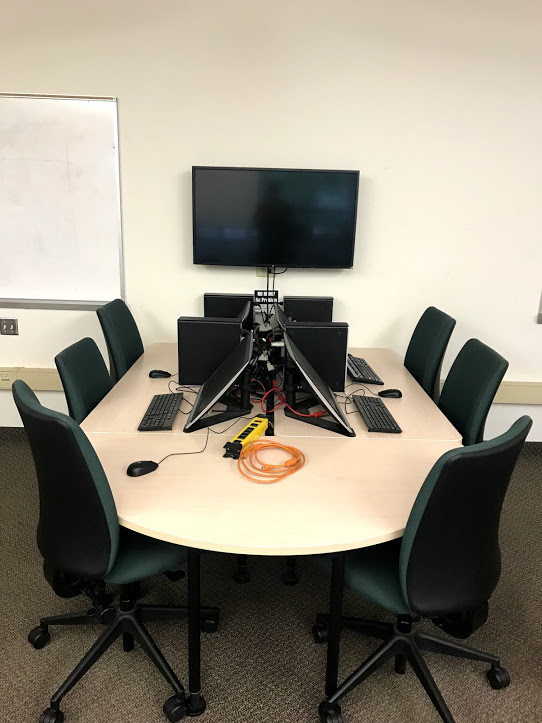
\includegraphics[scale=0.30]{images/1650Table.jpg}
   	\caption{Example Student Workstation}
   	\label{fig:RITResearchComputing}
\end{subfigure}%
\begin{subfigure}{.5\textwidth}
  \centering
 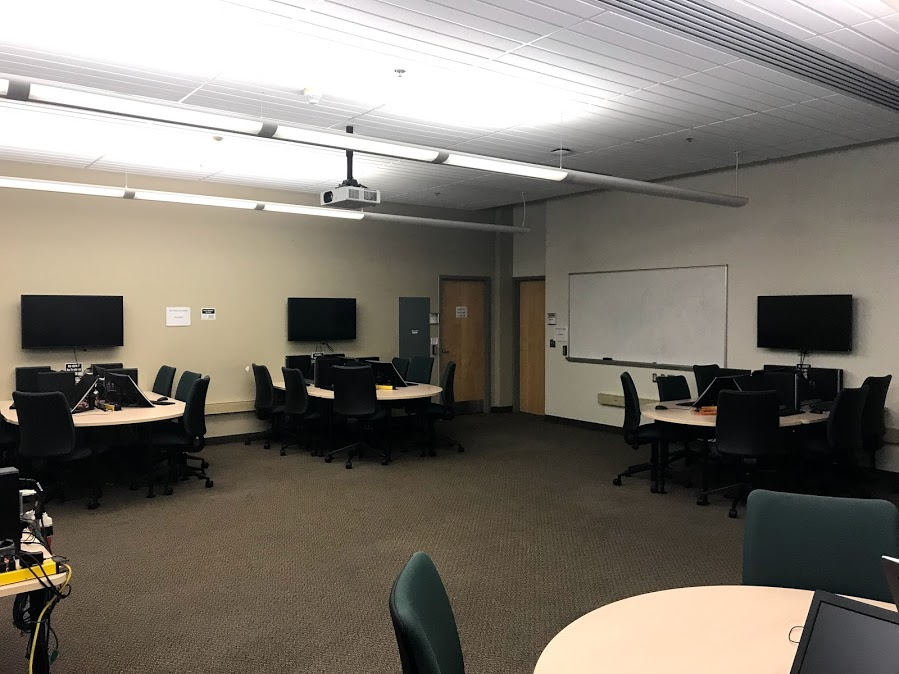
\includegraphics[scale=0.27]{images/1650Room.jpg}
    	\caption{Partial Room Overview}
   	\label{fig:RITDroneCage}
\end{subfigure}
\caption{Images of Classroom Space to be Used in Camp}
\label{fig:RITFacilities}
\end{figure}

% If space allows, maybe have an overhead diagram of the room. Develop this in powerpoint or something



\subsubsection{Residential Accommodations}
\dan{Get this from KoC}





%\subsection{Research Tasks} % Keep to about 1/2 page
%\label{sec: ResearchTasks}



\subsubsection{Kids on Campus Activities}
% Have been successfully used in many other camps
% Show students around the campus, answer questions
% Provide "Cybersecurity activities" that are disconnected
% KoC will provide chaperones/guidance
% Previous Gencyber offerings have shown us that this time is useful for getting particpants out of their seats and to expend energy


%Each day before lunch, students will be provided a `disconnected' activity where they will either be exposed to non-technology based security games, or be provided information about the `college experience' ie campus tours, discussions with admissions etc... The primary objective of these tours is not to merely promote RIT, but much more importantly familiarize the students with a college campus and the admissions process. We've found that this is especially important for many students who come from families 


Each day before lunch, students will be provided a `disconnected' activity where they may do things like CTF games, or security focused games. In at least one of these daily activities, students will be provided information about the `college experience' ie campus tours, discussions with admissions etc... The primary objective of these tours is not to merely promote RIT, but much more importantly familiarize the students with a college campus and help them to feel comfortable in a college setting. In previous camp offerings, we have observed that these types of `college experience' activities have been quite beneficial.% in making 



%Kids on Campus (KoC)


%


%%%%%%%%%%%%%%%%%%%%%%%%%%%%%%%%

\label{lastpage}
\cleardoublepage


%\appendix
%\addcontentsline{toc}{section}{Appendix}
%\begin{appendices}
%\chapter{Some Appendix}


%% DK: Put onto a different page since it does not count against the page limit
\setcounter{page}{1}

%\addcontentsline{toc}{subsection}{Project Schedule}
\cfoot{\thepage}
\pagenumbering{roman}
%\section{Appendix}

%\input{sections/Appendix.tex}



%% I think the appendix goes before the bib. Otherwise, I could see people missing it
\newpage
\pagebreak
\addcontentsline{toc}{section}{References}
\bibliographystyle{plain}
\bibliography{refs}


\end{document}

